\chapter{Frontend}
The frontend was made using React JS. In our frontend,we have separate interfaces for each tasks and we can easily navigate each of the interfaces through the navbar. Also, we can also toggle between light mode and dark mode too. Keeping in mind about the user experience, we have also made the cursor appear inside the textbox without needing the user to click inside the textbox to type. The text typed inside the text box gets transliterated to nepali language for which we used \textbf{Google Input Tools Transliteration API}. This makes user able to type directly in nepali langauge and perform specific actions without need of any external tools for providing nepali language input. We have also made the UI as simple as possible and presented options in a visible way so users don’t have to remember where they are and what they are able to do. We have also made use of proper mouse pointers as well to let the user know when they are able to click certain button and when they are not. We have kept the screens and dialogues focused and minimal to maximize visibility and clarity and used terminology and language familiar to the user. 

Our default mode is light mode and default interface/page is home page. 

\begin{figure}[H]
    \centering
    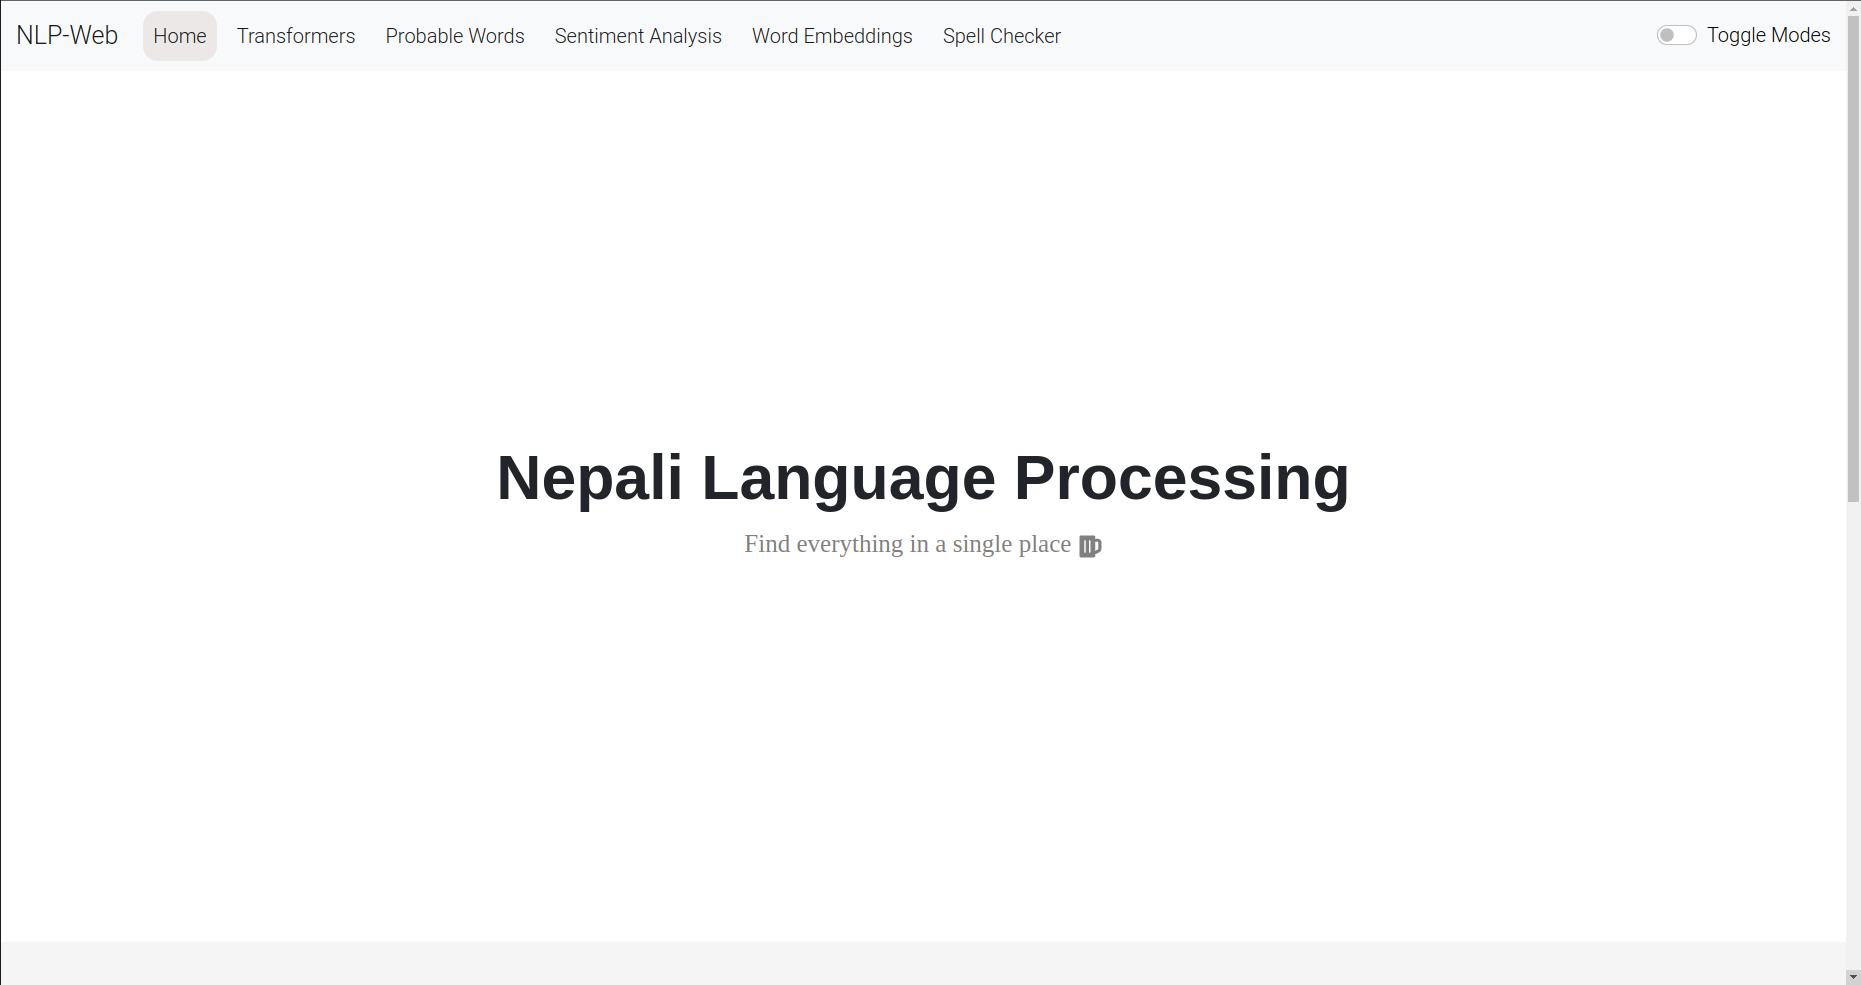
\includegraphics[scale = 0.25]{frontend/home_frontend.png}
    \caption{Homepage Light Mode}
    \label{fig: Homepage Light Mode}
\end{figure}


% \begin{figure}[H]
%     \centering
%     \includegraphics[scale = 0.35]{frontend/home_dark.png}
%     \caption{Homepage Dark Mode}
%     \label{fig: Homepage Dark Mode}
% \end{figure}

We can navigate to transformer through navbar which provides you with an interface that lets you to see the text generated based on your input text and number of words to be generated. By default the number of words is set to 3, with freedom for user to change it if they want as they like. Just after giving all the inputs as you like, you can now press the button. The request is then sent to the API of our backend and the response is displayed as shown in the figure below.

\begin{figure}[H]
    \centering
    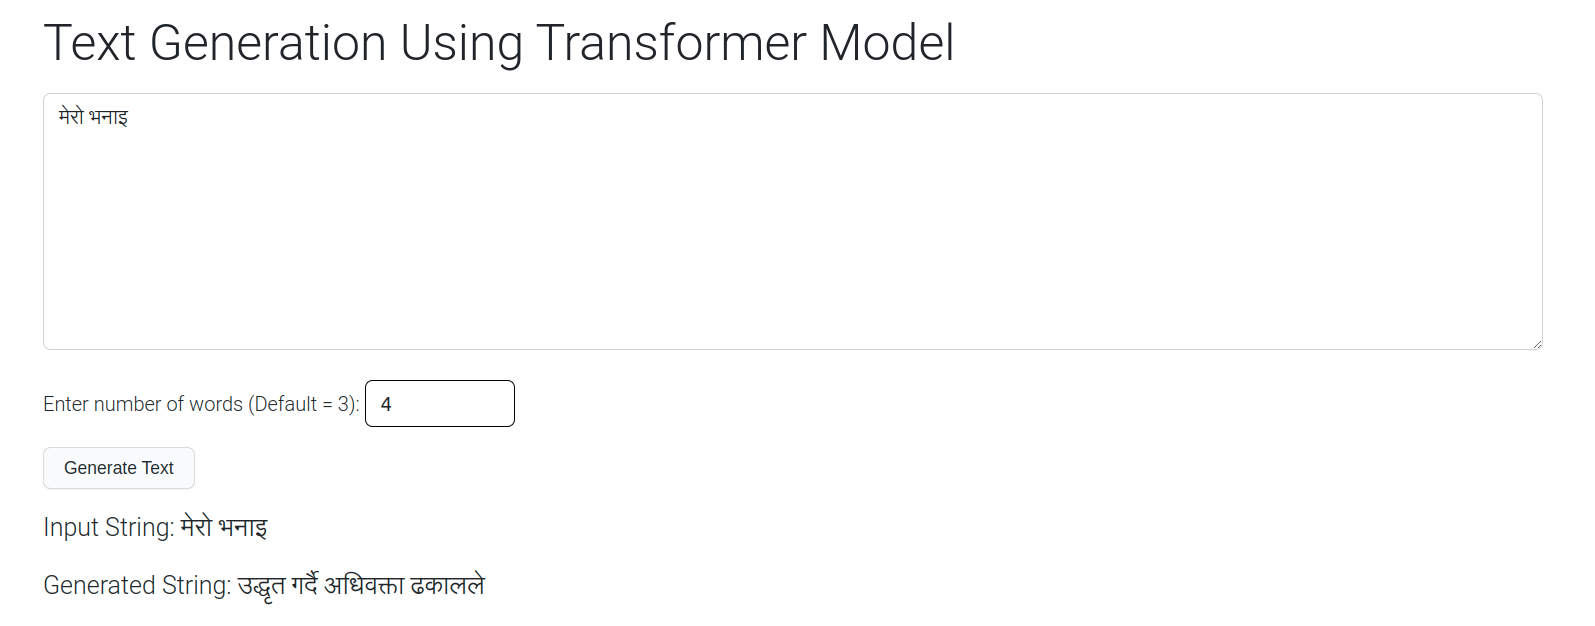
\includegraphics[scale = 0.3]{frontend/transformer_frontend.png}
    \caption{Transformer based LM Frontend}
    \label{fig: Transformer based LM Frontend}
\end{figure}

Likewise, we can navigate to Probable words through navbar which provides you with an interface that lets you input text in text field where you can directly type just after navigating to it through navbar.  The request is sent to the API of our backend and the response is displayed as shown in the figure below. Now just as before, enter the text you like and  press the button. The request is then sent to the API of our backend. Based on the response, the probabilty if the next 5 possible text with their probabilty are shown in the table along with their visualization with the help of progress bar.

\begin{figure}[H]
    \centering
    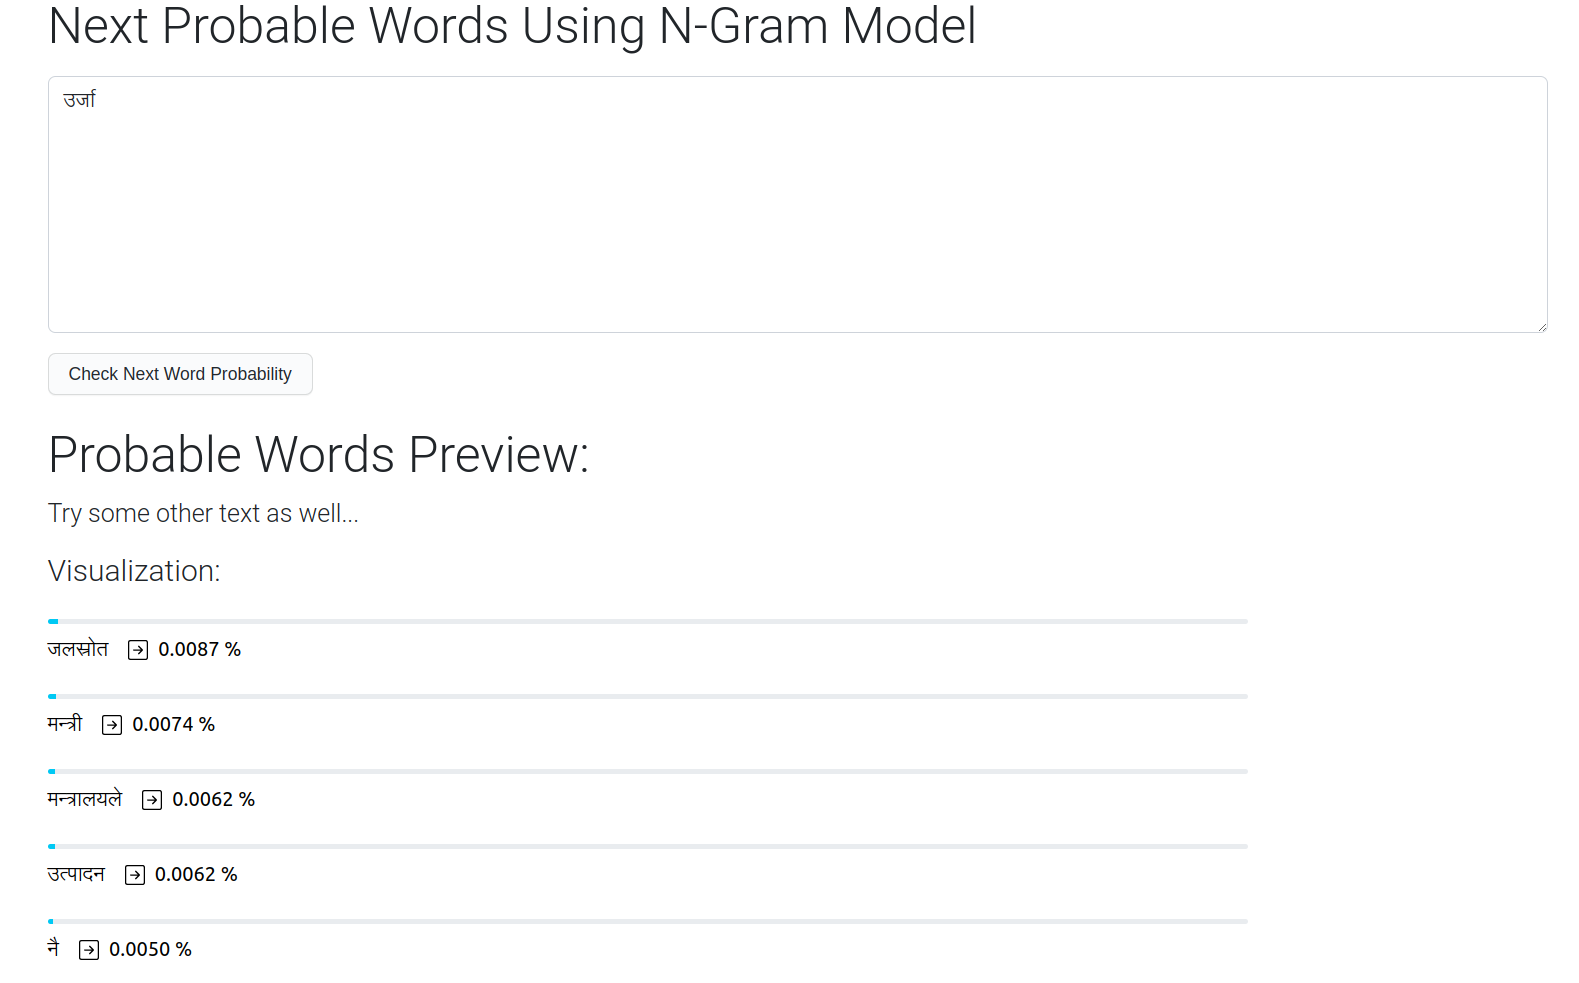
\includegraphics[scale = 0.3]{frontend/probabilistic_frontend.png}
    \caption{Proabilistic Language Model Frontend}
    \label{fig: Proabilistic LM Frontend}
\end{figure}

Similarly, you will get another interface after navigating to sentiment anlysis. The sentiment type of given text is displayed after you click the button along with the probabilty of its sentiments with progress bar.

\begin{figure}[H]
    \centering
    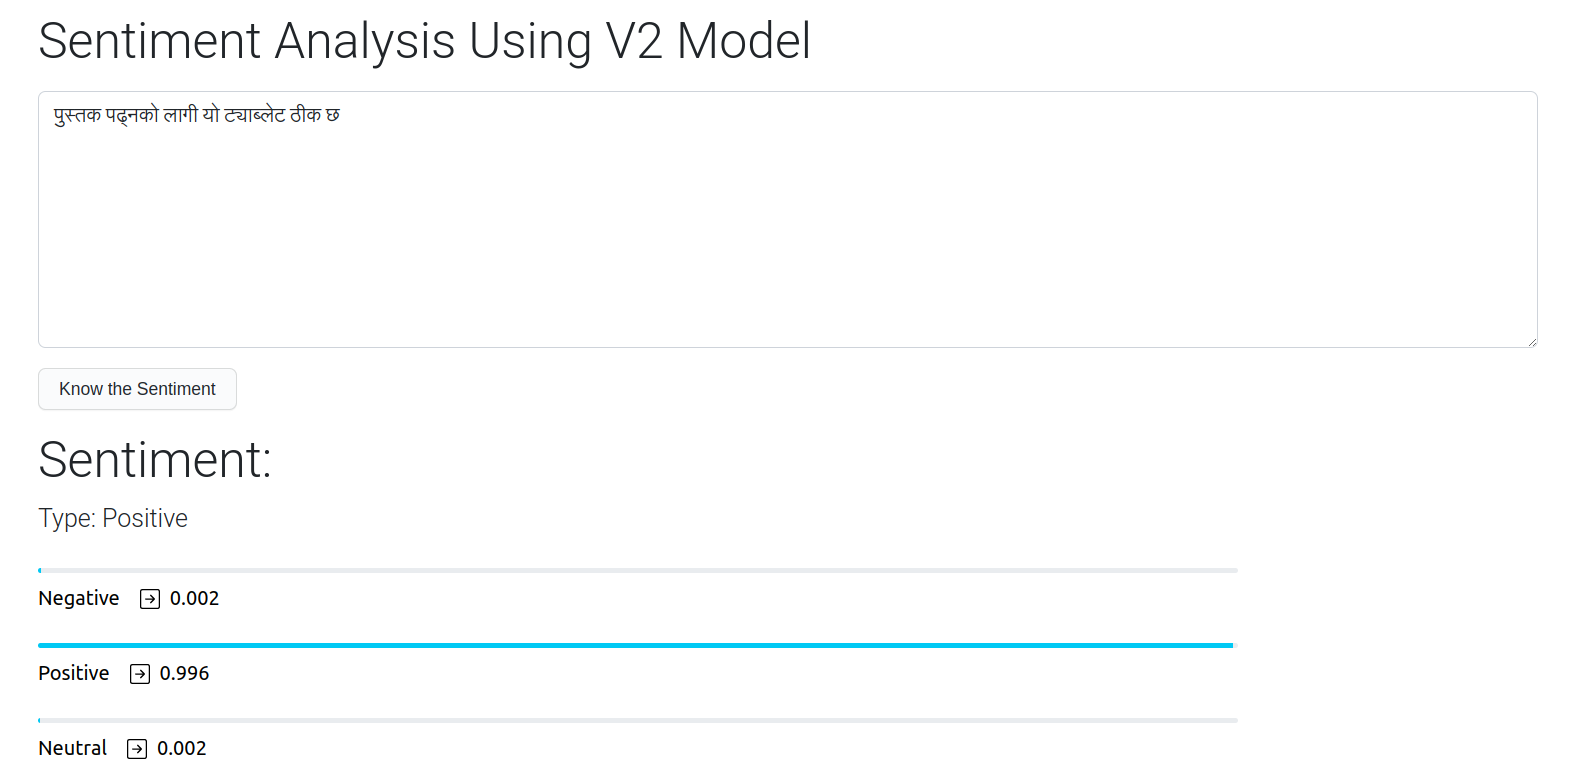
\includegraphics[scale = 0.3]{frontend/positive_sentiment.png}
    \caption{Positive Sentiment Prediction}
    \label{fig: Positive Sentiment Prediction}
\end{figure}

\begin{figure}[H]
    \centering
    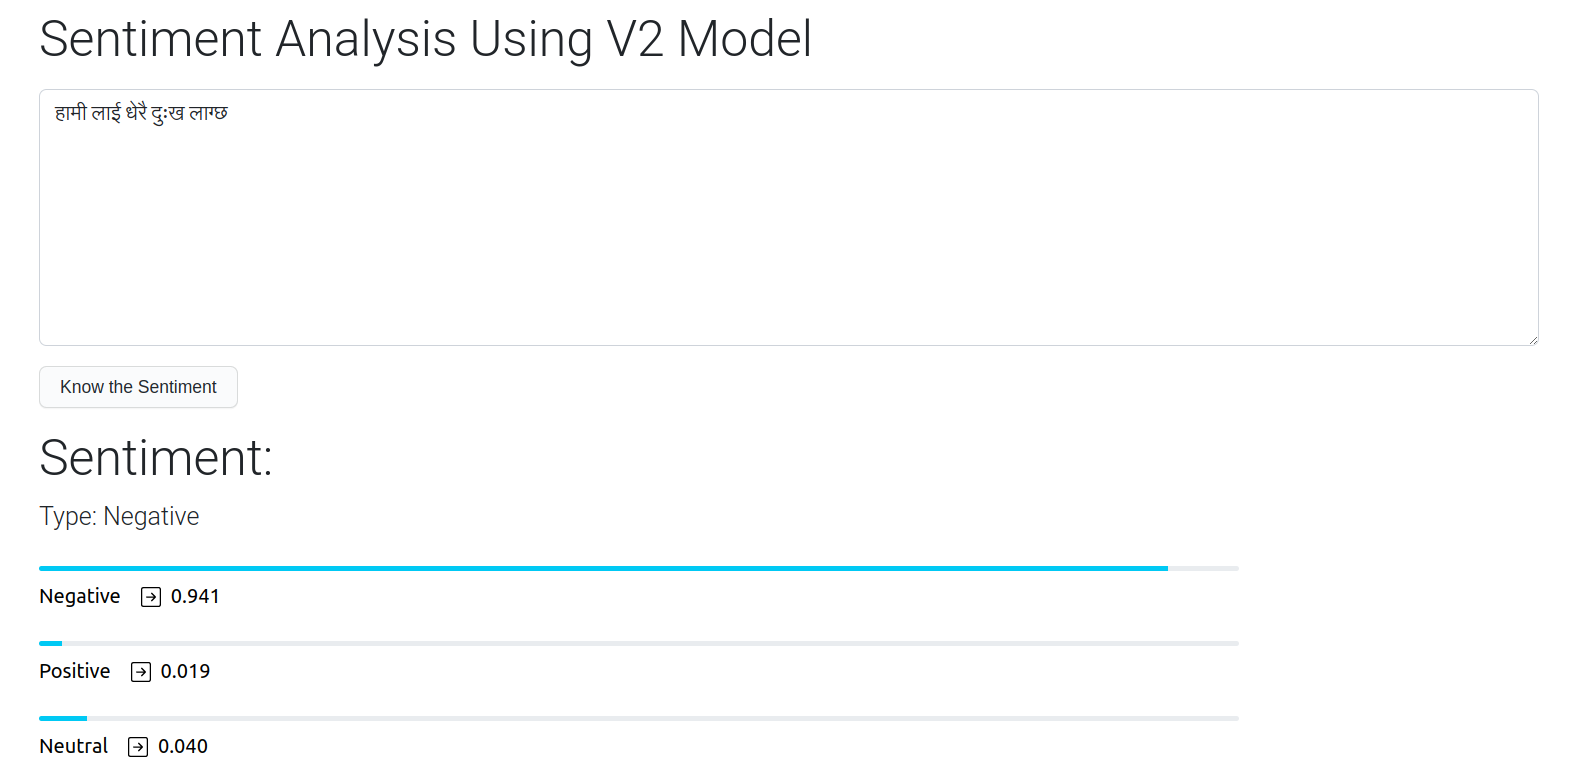
\includegraphics[scale = 0.3]{frontend/negative_sentiment.png}
    \caption{Negative Sentiment Prediction}
    \label{fig: Negative Sentiment Prediction}
\end{figure}

\begin{figure}[H]
    \centering
    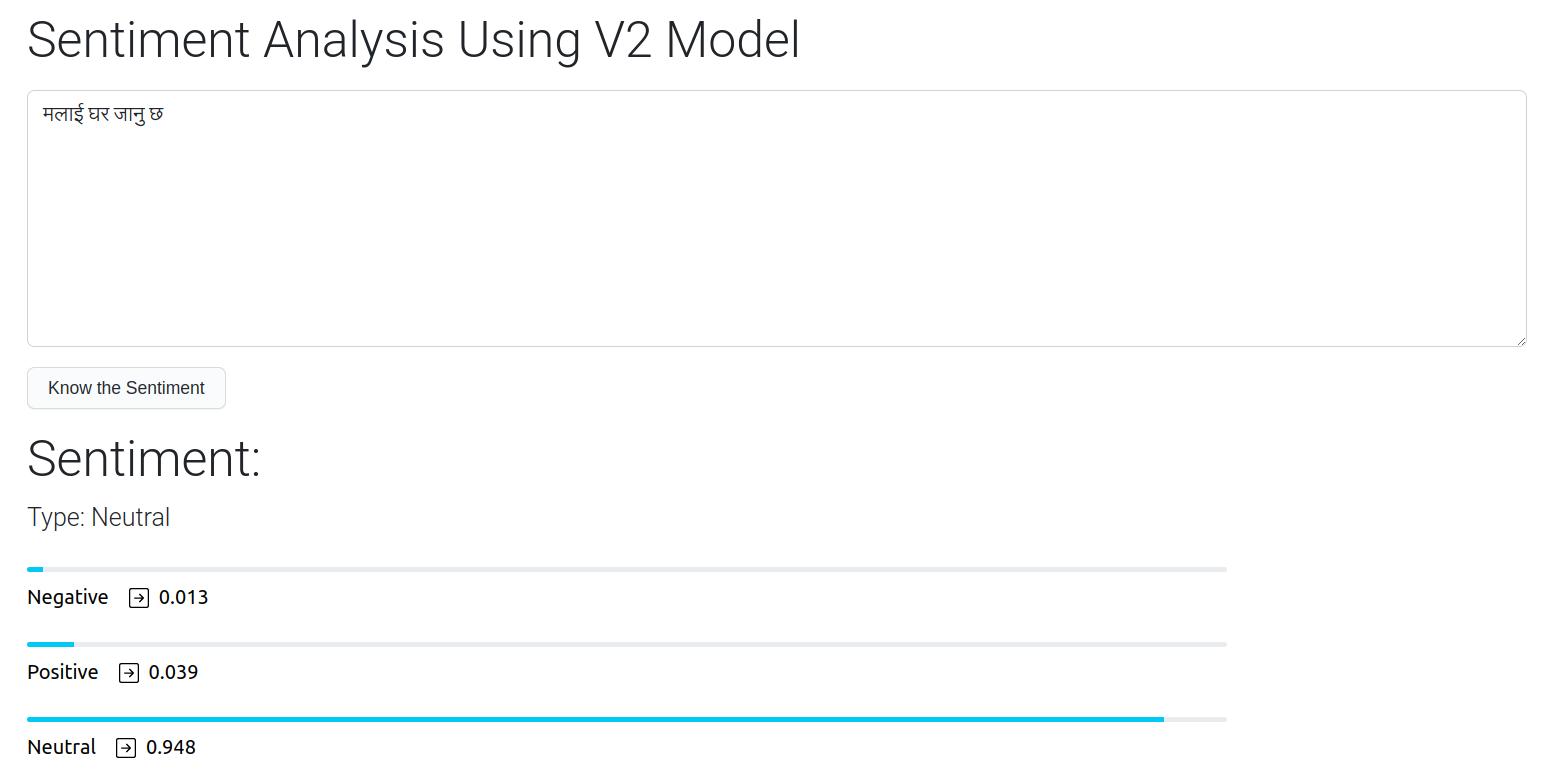
\includegraphics[scale = 0.3]{frontend/neutral_sentiment.png}
    \caption{Neutral Sentiment Prediction}
    \label{fig: Neutral Sentiment Prediction}
\end{figure}



In word embeddings you can either choose to see 2d or 3d word embeddings visualization graph just by clicking buttons. The 2d graph is made using the canvs.js graphing library and 3d graph is made using plotly.js library.

\begin{figure}[H]
    \centering
    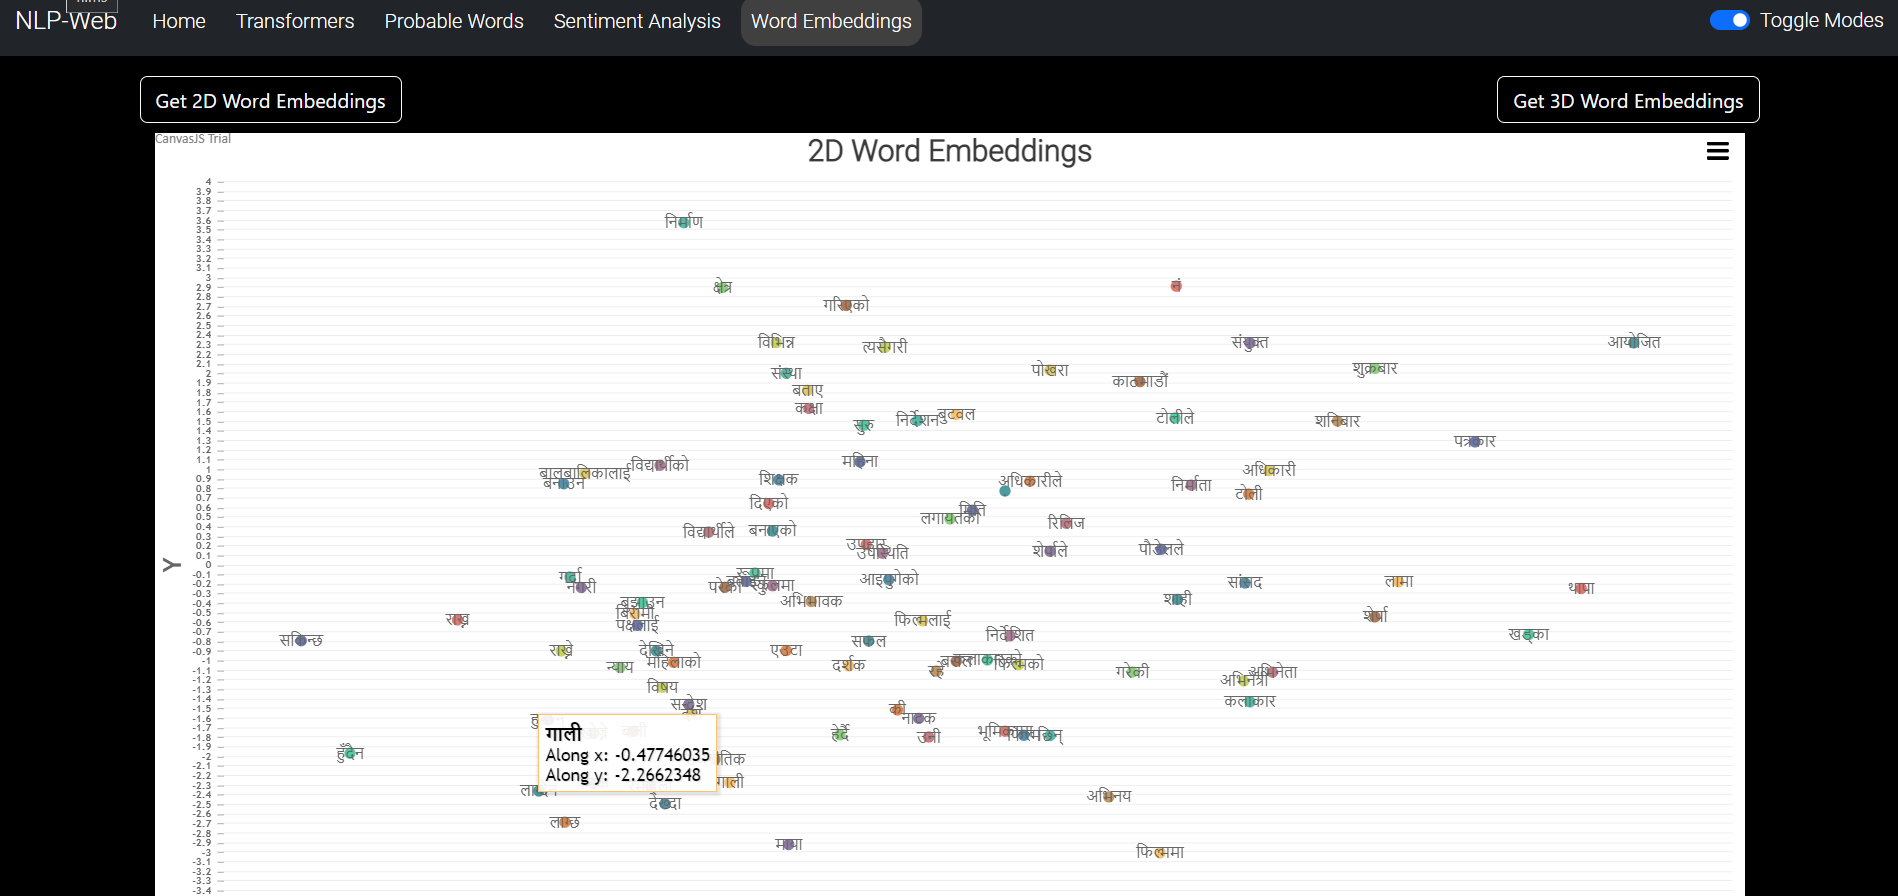
\includegraphics[scale = 0.35]{frontend/word_embedding_2d.png}
    \caption{Word Embedding 2d plot Frontend}
    \label{fig: Word Embedding 2d plot Frontend}
\end{figure}

\begin{figure}[H]
    \centering
    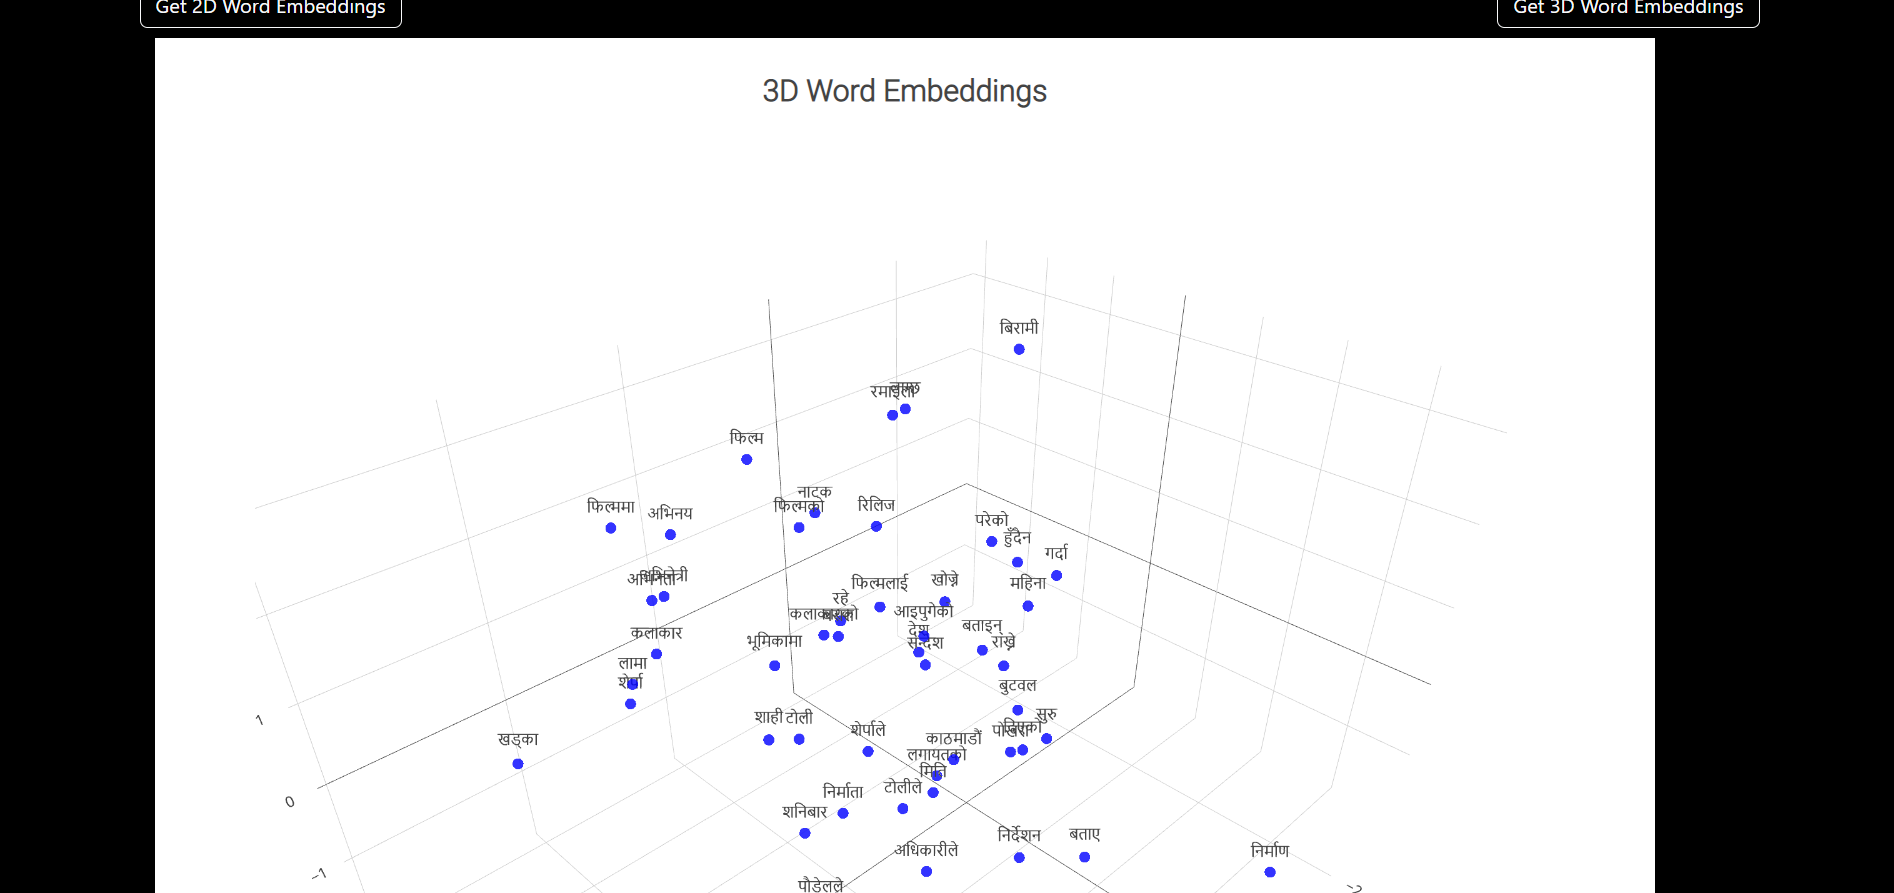
\includegraphics[scale = 0.35]{frontend/word_embedding_3d.png}
    \caption{Word Embedding 3d plot Frontend}
    \label{fig: Word Embedding 3d plot Frontend}
\end{figure}

In spell checker, we can get auto corrected output of the given text. In addition to that, we can also manually correct the text  based on the choices provided. By manually choosing the choices provided for each text, the spelling correction is more likely to be accurate. Below is the screenshot for spelling correction.

\begin{figure}[H]
    \centering
    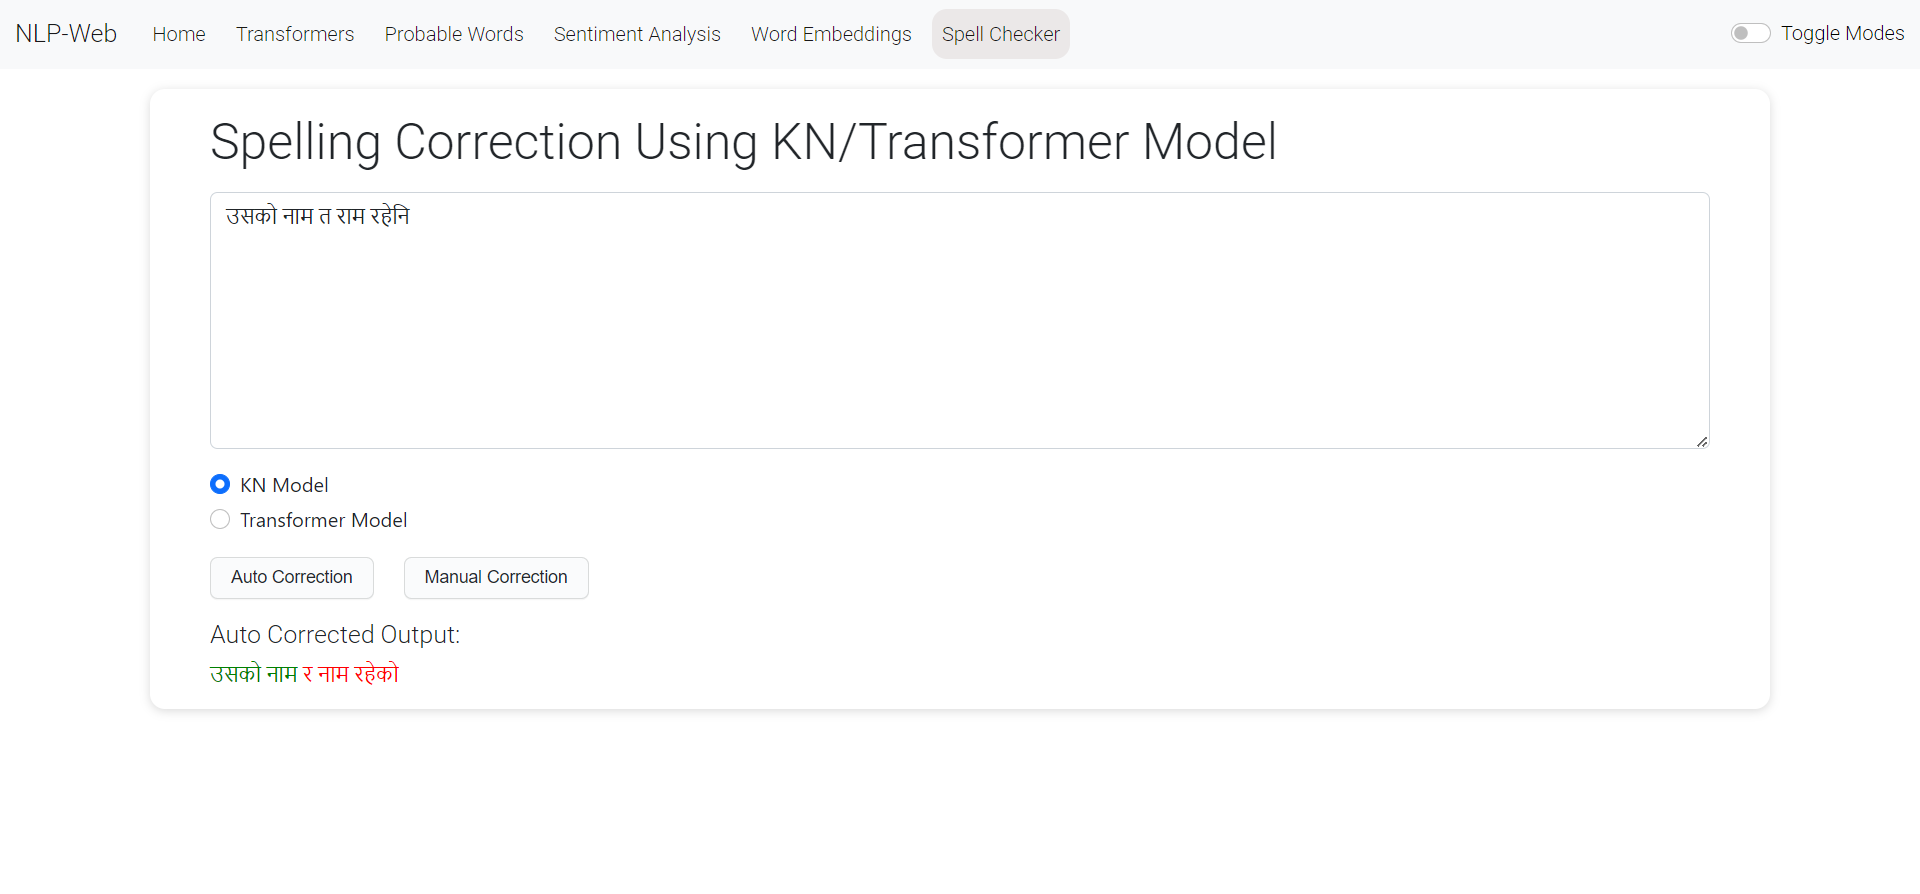
\includegraphics[scale = 0.25]{frontend/kn_model.png}
    \caption{Auto Spelling Correction}
    \label{fig: Auto Spelling Correction}
\end{figure}

\begin{figure}[H]
    \centering
    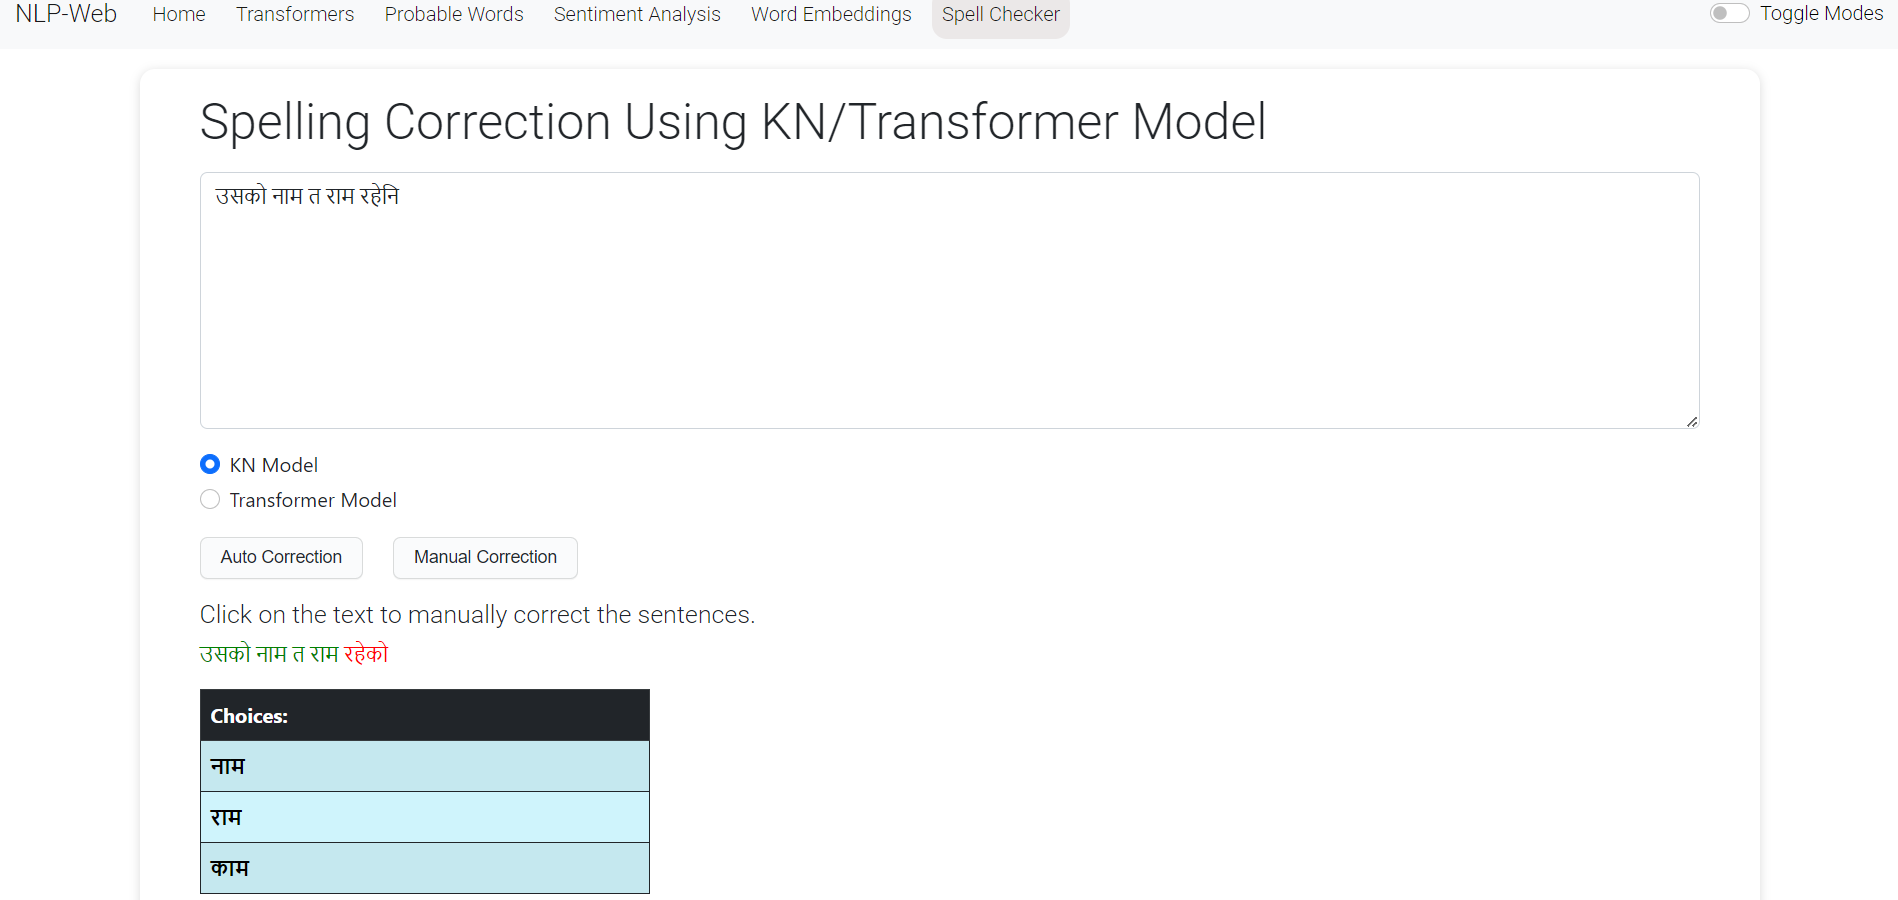
\includegraphics[scale = 0.25]{frontend/manual_correction.png}
    \caption{Manual Spelling Correction}
    \label{fig: Manual Spelling Correction}
\end{figure}
